\documentclass[tikz]{standalone}
\usepackage{tikz}
\usepackage{soul}
\usetikzlibrary{arrows.meta, positioning, calc}

\begin{document}
	
	
	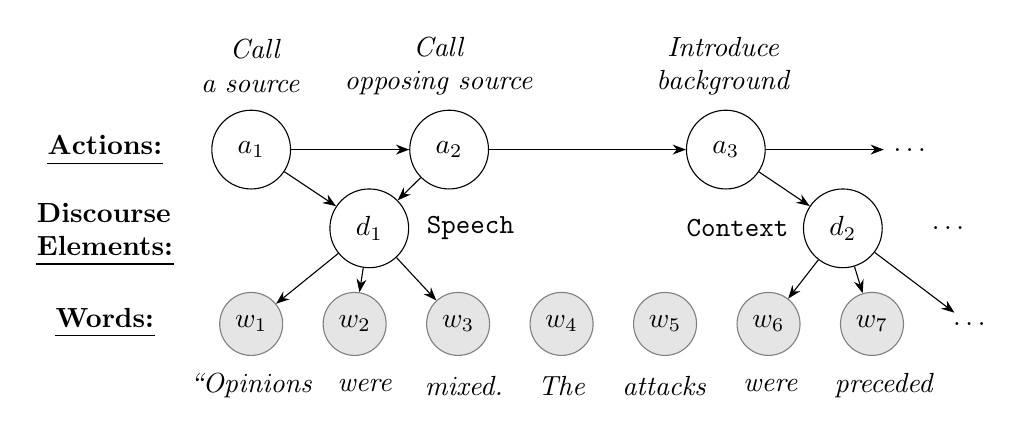
\begin{tikzpicture}[node distance=1cm, auto, >=Stealth]
		
		% Styles for nodes
		\tikzstyle{action} = [circle, draw=black, minimum size=1cm]
		\tikzstyle{discourse} = [circle, draw=black, minimum size=1cm]
		\tikzstyle{word} = [circle, draw=gray, fill=gray!20, minimum size=0.8cm]
		\tikzstyle{ellipsis} = [node distance=1cm]
		
		% Top row: Actions
		\node[action] (a1) {$a_1$};
		\node[action, right=1.5cm of a1] (a2) {$a_2$};
		\node[action, right=2.5cm of a2] (a3) {$a_3$};
		\node[ellipsis, right=1.5cm of a3] (adots) {$\dots$};
		
		% Label each row
%		\node[left=0.5cm of a1, align=left] (l1){\textbf{Actions/}\\ \textbf{\ul{Intentions:}}};
		\node[left=0.5cm of a1, align=left] (l1){\textbf{\ul{Actions:}}};
		\node[below=.25cm of l1, align=left] (l2){\textbf{Discourse} \\ \textbf{\ul{Elements:}}}; % \\ \textbf{\ul{Elements:}}};
		\node[below=.3cm of l2, align=left] {\textbf{\ul{Words:}}};
		
		% Labels above actions
		\node[above=0.1cm of a1, align=center](al1){\textit{ Call} \\ \textit{a source}};
		\node[right=.3cm of al1, align=center](al2){\textit{Call} \\ \textit{opposing source}};
		\node[right=1.3cm of al2, align=center] (al3){\textit{Introduce} \\ \textit{background}};
		
		% Middle row: Discourse
		\node[discourse] (d1) at ($(a1) + (1.5cm, -1cm)$) {$d_1$};
		\node[discourse, right=5cm of d1] (d2) {$d_2$};
		\node[ellipsis, right=.5cm of d2] (ddots) {$\dots$};
		
		% labels next to discourse
		\node[right=0.1cm of d1, align=left] {\texttt{Speech}};
		\node[right=3.4cm of d1, align=left] {\texttt{Context}};
		
		% Bottom row: Words
		\node[word, below=1.3cm of a1] (w1) {$w_1$};
		\node[word, right=.5cm of w1] (w2) {$w_2$};
		\node[word, right=.5cm of w2] (w3) {$w_3$};
		\node[word, right=.5cm of w3] (w4) {$w_4$};
		\node[word, right=.5cm of w4] (w5) {$w_5$};
		\node[word, right=.5cm of w5] (w6) {$w_6$};
		\node[word, right=.5cm of w6] (w7) {$w_7$};
		\node[ellipsis, right=.5cm of w7] (wdots) {$\dots$};
		
		% Connections between action nodes
		\draw[->] (a1) -- (a2);
		\draw[->] (a2) -- (a3);
		\draw[->] (a3) -- (adots);
		
		% Connections from actions to discourse
		\draw[->] (a1) -- (d1);
		\draw[->] (a2) -- (d1);
		\draw[->] (a3) -- (d2);
				
		% Connections from discourse to words
		\draw[->] (d1) -- (w1);
		\draw[->] (d1) -- (w2);
		\draw[->] (d1) -- (w3);
		
		\draw[->] (d2) -- (w6);
		\draw[->] (d2) -- (w7);
		\draw[->] (d2) -- (wdots);
		
		\node[below=0.1cm of w1, align=left] (wl1) {\textit{``Opinions}};
		\node[right=.05cm of wl1, align=left] (wl2){\textit{were}};
		\node[right=.15cm of wl2, align=left](wl3) {\textit{mixed.}};
		\node[right=.2cm of wl3, align=left](wl4) {\textit{The}};
		\node[right=.2cm of wl4, align=left](wl5) {\textit{attacks}};
		\node[right=.2cm of wl5, align=left](wl6) {\textit{were}};
		\node[right=.2cm of wl6, align=left](wl7) {\textit{preceded}};
	\end{tikzpicture}
	
\end{document}
